\section{Scattering in QED}
\subsection{LSZ for Fermions}
Today we move to the last big topic in QFT II! We'll derive the LSZ formula for Dirac fermion and photons. We will go back to our Hamiltonian expressions to derive it, and then after deriving, compute the S-matrix amplitudes via path integrals.

We recall the solutions to the Dirac equation found via mode expansion:
\begin{equation}
    \psi(x) = \sum_{s=\pm}\int \frac{d^3p}{(2\pi)^32\e_{\v{p}}}[b_{s, \v{p}}u_s(\v{p})e^{ipx} + d^\dag_{s, \v{p}}v_s(\v{p})e^{-ipx}]
\end{equation}
with:
\begin{equation}
    u_s(\v{0}) = \sqrt{m}\m{1\\0\\1\\0}, \quad
\end{equation}
and:
\begin{equation}
    \set{b_{s\v{p}}, b_{s'\v{p}'}} = 2\e_{\v{p}}(2\pi)^3\delta^3(\v{p} - \v{p}')\delta_{ss'}
\end{equation}
We also inverted these equations to get $b/d$ in terms of the quantum field $\psi$:
\begin{equation}\label{eq:bdagddag}
    \begin{split}
        b^\dag_{s, \v{p}} &= \int d^3xe^{ipx}\bar{\psi}(x)\gamma^0 u_s(\v{p})
        \\ d^\dag_{s, \v{p}} &= \int d^3x e^{ipx}\bar{v}_s(\v{p})\gamma^0 \psi(x)
    \end{split}
\end{equation}
Note the time dependence present in the exponential (with $p^0 = \e_p = \sqrt{\v{p}^2 + m^2}$) gets cancelled with the time dependent part of $\psi$ to make the overall expressions time-independent.

In the free theory, these operators are time-independent, and these operators create single-particle states:
\begin{equation}
    \begin{split}
        b^\dag_{s, \v{p}} &= \ket{\v{p}, s, e}
        \\ d^\dag_{s, \v{p}} &= \ket{\v{p}, s, -e}
    \end{split}
\end{equation}
In the free theory, these states are boring - the states are time-independent and nothing happens to them. In the interacting theory, we would like to build scattering states. The $b^\dag_{s, \v{p}}(t)$ and $d^\dag_{s, \v{p}}(t)$ defined via Eq. \eqref{eq:bdagddag} will have time-dependence in the interacting theory (because we don't know how $e^{iHt}$ acts in the interacting theory). Put another way:
\begin{equation}
    b^\dag_{s, \v{p}}(t) \ket{0} \neq b^\dag_{s, \v{p}}(t') \ket{0}
\end{equation}
for $t \neq t'$. We want to construct single-particle states for early and late times. The intuition is that at a specific time, $b^\dag_{s, \v{p}}(t) \ket{0}$ ``looks'' like a single-particle state, even though it may time evolve nontrivially.

So - our states that are simple at asymptotically early times (the ``in'-states here for two fermions) are:
\begin{equation}
    \ket{i} = b^\dag_{s_1, \v{p}_1}(-\infty)b^\dag_{s_2, \v{p}_2}(-\infty)\ket{0}
\end{equation}
And the states that are simple at late times (the ``out''-states) are:
\begin{equation}
    \ket{f} = b^\dag_{s_3, \v{p}_3}(\infty)b^\dag_{s_4, \v{p}_4}(\infty)\ket{0}
\end{equation}
The reason this works is that even though we have not identified the true multi-particle states, our guess has some overlap with the true multi-particle states.
\begin{equation}
    \bra{\v{p}, s, e}b^\dag_{s, \v{p}}\ket{0} \neq 0
\end{equation}
so we may appropriately normalize and use our ansatz as the in/out states. The intuition is that well-separated wavepackets are non-interacting.

We also require that overlap with multiparticle states vanishes:
\begin{equation}
    \bra{\v{p}, s, \v{p}', s'}b^\dag_{s, \v{p}}(-\infty)\ket{0} = 0
\end{equation}
this crucially hinges on the existence of a finite mass gap between the single particle states and the multi-particle continuum. Indeed this will cause trouble in QED, as though the electrons have mass, the photons are massless.

\begin{center}
    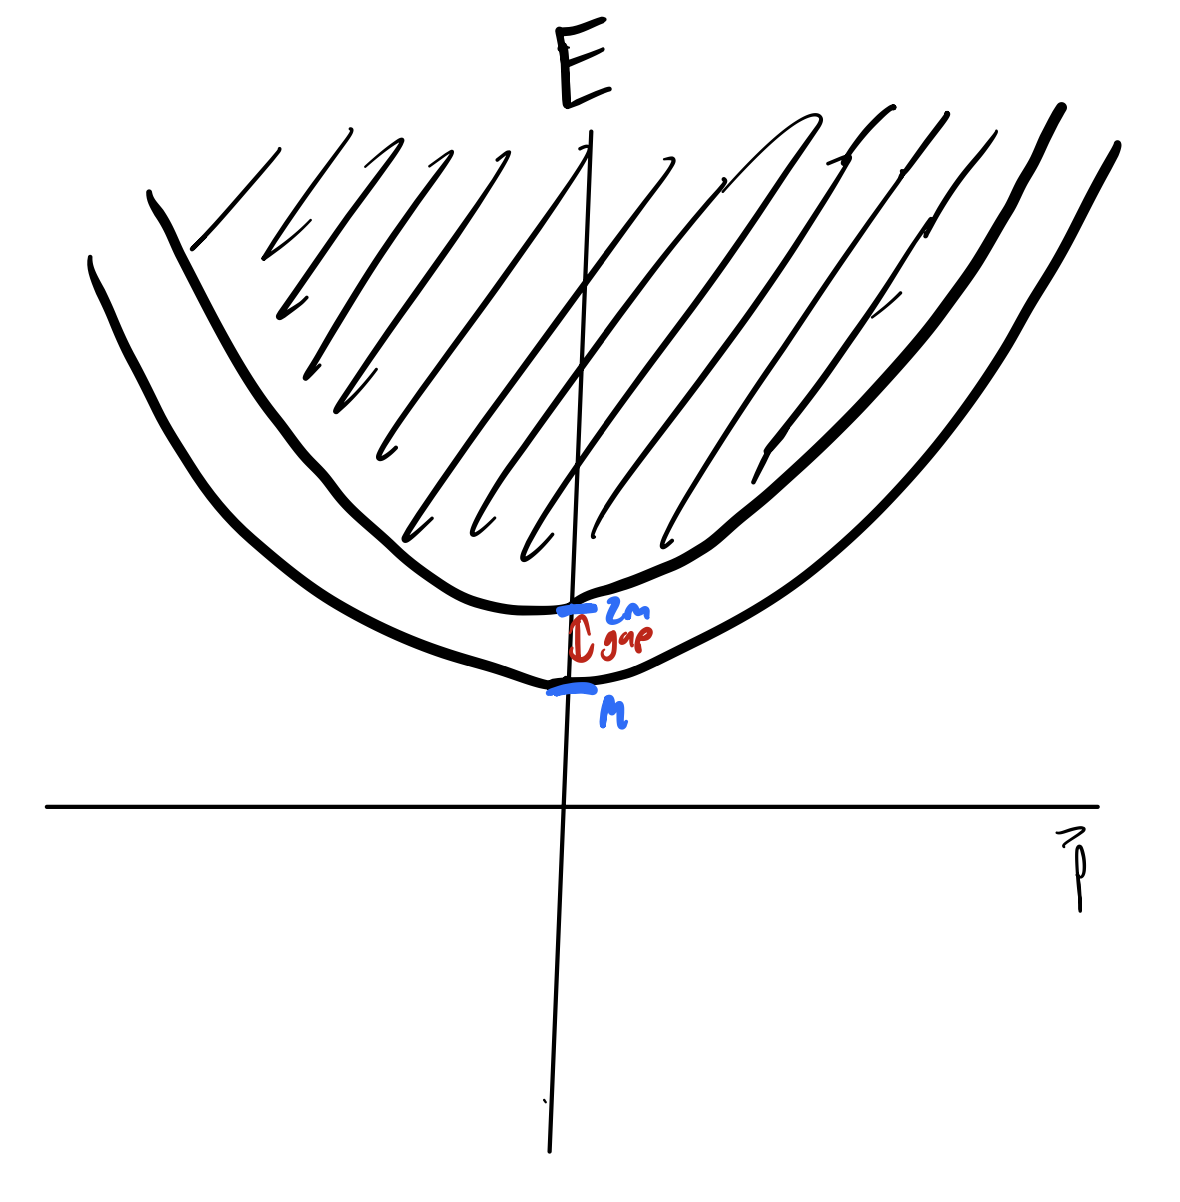
\includegraphics[scale=0.35]{Lectures/Images/lec12-massgap.png}
\end{center}

So, let's find a formula for the probability that a given in state goes to a given out state, $p(i\to f)$, given by the (square of) the matrix elements $S_{fi} = \bra{f}{i}$. As for the scalar field, we work out the difference between two creation operators:
\begin{equation}
    \begin{split}
        b^\dag_{s, \v{p}}(\infty) - b^\dag_{s, \v{p}}(-\infty) &= \int_{-\infty}^\infty dt \p_t b_{s, p}
        \\ &= \int d^4x \p_t(e^{ipx}\bar{\psi}(x)\gamma^0u_s(\v{p}))
        \\ &= \int d^4x e^{ipx}(ip_0 + \p_0)\bar{\psi}(x)\gamma^0u_s(\v{p})
    \end{split}
\end{equation}
the above equation reminds us of $(\slashed{p} + m)u_s(\v{p}) = 0$, so then:
\begin{equation}
    b^\dag_{s, \v{p}}(\infty) - b^\dag_{s, \v{p}}(-\infty) = \int d^4x\bar{\psi}(\overleftarrow{\p_0} \gamma^0 - ip_i \gamma^i - im)u_s(\v{p})e^{ipx}
\end{equation}
If we now integrate by parts (in space); we can replace $ip_i = \overrightarrow{\p_i}$ with $-\overleftarrow{\p_i}$ and so:
\begin{equation}
    \begin{split}
        b^\dag_{s, \v{p}}(\infty) - b^\dag_{s, \v{p}}(-\infty) &= \int d^4x \bar{\psi}(\overleftarrow{\slashed{p}} - im)u_s(\v{p})e^{ipx}
        \\ &= -i\int d^4x \bar{\psi}(i\overleftarrow{\slashed{p}} + m)u_s(\v{p})e^{ipx}
    \end{split}
\end{equation}
Taking the conjugate of this expression, we similarly find:
\begin{equation}
    b_{s, \v{p}}(\infty) - b_{s, \v{p}}(-\infty) = i\int d^4x e^{-ipx}\bar{u}_s(\v{p})(-i\slashed{\p} + m)\psi
\end{equation}
So now we did the same thing we did for our scalar field theory. We plug these expressions into the expression for the $S$-matrix elements:
\begin{equation}
    \braket{f}{i} = \bra{0}\mathcal{T}b_{s_3, \v{p}_3}(\infty)b_{s_4, \v{p}_4}(\infty)b^\dag_{s_1, \v{p}_1}(-\infty)b^\dag_{s_2, \v{p}_2}(-\infty)\ket{0}
\end{equation}
where we have introduced a time-ordering operator for free - we can now replace the $b^\dag, b$s with the differences that we computed above, which are equivalent due to the time ordering (time ordering kills the other terms by virtue of $b\ket{0} = \bra{0}b^\dag = 0$ - the mass gap assumption guarantees that the annihilation operators still annihilate the vacuum of the theory). We are left with:
\begin{equation}
    \begin{split}
        \braket{f}{i} = i^4\int_{x_1x_2x_3x_4}&e^{-ip_3x_3 - ip_4x_4}[\bar{u}_{s_3p_3}(-i\slashed{\p}_{x_3} + m)]_{\alpha}[\bar{u}_{s_4p_4}(-i\slashed{p}_{x_4} + m)]_{\beta}\bra{0}\mathcal{T}\psi_{\alpha}(x_3)\psi_{\beta}(x_4)\bar{\psi}_{\gamma}(x_1)\bar{\psi}_{\delta}(x_2)\ket{0}
        \\ &\cdot [(i\overleftarrow{\slashed{\p}}_{x_1} + m)u_{s_1}(\v{p}_1)]_\gamma[(i\overleftarrow{\slashed{\p}}_{x_2} + m)u_{s_2}(\v{p}_2)]_\delta e^{ip_1x_1 + ip_2x_2}
    \end{split}
\end{equation}
This looks complicated, but the extra factors actually end up being useful - they amputate the external propagators and put the particle on-shell. This condition drastically reduces the dependencies on the variables - for the scalar case we reduced things to Mandelstam variables $s, t, u$ (only of which 2 were independent), and although things are more complicated here due to the presence of spin indices, again things will simplify.

\begin{center}
    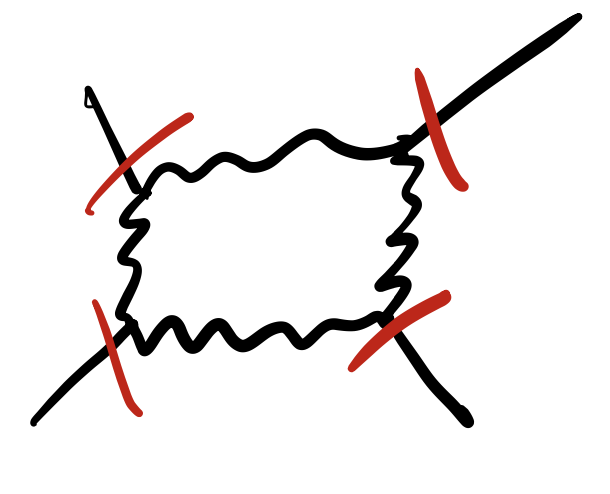
\includegraphics[scale=0.35]{Lectures/Images/lec12-amputatedlegs.png}
\end{center}

The expression actually looks much simpler in momentum space. Like for scalars $\braket{f}{i} = \delta_{if} + T_{if}$, we can use momentum conservation to write:
\begin{equation}
    iT_{if} = (2\pi)^4\delta^4(p_1 + p_2 - p_3 - p_4)i\mathcal{M}(p_1p_2 \to p_3p_4)
\end{equation}
which leaves us with:
\begin{equation}
    \begin{split}
        &i\mathcal{M}(p_1p_2 \to p_3p_4) = 
        \\ &[\bar{u}_{s_3}(\v{p}_3)(\slashed{p}_3 + m)]_\alpha [\bar{u}_{s_4}(\v{p}_4)(\slashed{p}_4 + m)]_\beta \avg{\mathcal{T}\psi_{\alpha}(\v{p}_3)\psi_{\beta}(\v{p}_4)\bar{\psi}_\gamma(\v{p}_1)\bar{\psi}_\gamma}_c [(\slashed{p}_1 + m)u_{s_1}(\v{p_1})]_\gamma[(\slashed{p}_2 + m)u_{s_2}(\v{p_2})]_\delta
    \end{split}
\end{equation}
where we see that the expressions in brackets $[\cdot]$ are just the inverse propagators, which amputate the external legs.

\subsection{LSZ for photons}
We saw that photons have two propagating degrees of freedom, which we labelled with helicity $\pm 1$. We expect naively:
\begin{equation}
    \braket{\ldots}{\v{p}, h} = \e^h_\mu (p^2\eta^{\mu\nu} + (\xi - 1)p^\mu p^\nu)\avg{\mathcal{T}A_\nu\ldots}
\end{equation}
Naively, it looks like we could choose 4 polarizations, $\e_\mu = \delta_\mu^0, \delta^x_\mu, \delta^y_\mu, \delta^z_\mu$. We will see that due to Gauge invariance, only two polarizations are physical.

Let's set $p^\mu = (p, 0, 0, p)$, with $p^z = p^0$, and $(p^\mu)^2 = 0$ as required. Helicity is an eigenvalue under $J_3$ with this choice. Now consider $\e^{(x)}_\mu = \delta^x_\mu$ and $\e^{(y)}_\mu = \delta^y_\mu$. These vectors get exchanged under $J_2$ rotation:
\begin{equation}
    \m{\e^{(x)} \\ \e^{(y)}} \to \m{\cos\theta & \sin\theta \\ -\sin\theta & \cos\theta}\m{\e^{(x)} \\ \e^{(y)}}
\end{equation}
So we have the eigenvectors $\e^\mp_\mu = \e^{(x)}_\mu \mp i\e^{(y)}_\mu$; to see this:
\begin{equation}
    \e^{(x)}_\mu \mp i\e^{(y)}_\mu \mapsto \cos\theta \e^{(x)} + \sin\theta \e^{(y)} \mp i(\cos\theta \e^{(y)}  - \sin\theta \e^{(x)}) = (\cos\theta \pm i\sin\theta)(\e^{(x)} \mp i\e^{(y)}) = e^{\pm i\theta}\e^{\mp}
\end{equation}
These are the states we expect to be physical. They have an important property that they are orthogonal to the wavevector:
\begin{equation}
    \e^{\pm}_\mu p^\mu = 0
\end{equation}
which tells us that this is gauge invariant. One way to be orthogonal to $p^\mu$ is to take $p_\mu$, but $\e^\pm_\mu$ are \emph{not} the null vector; they are vectors orthogonal in the Minkowski metric that are orthogonal to momentum without being the momentum itself.

Our guess for the LSZ formula thus simplifies (as the gauge dependent part gets killed):
\begin{equation}
    \braket{\ldots}{\v{p}, h} = \e^h_\mu p^2\avg{\mathcal{T}A^\mu\ldots}
\end{equation}
What happens to the other polarizations? They do produce physical states, but correspond to the pure gauge component $A_\mu \sim \p_\mu \lambda$ and the constrained variable.
\begin{equation}
    \e^\mu_1 = (1, 0, 0, 1) \propto p^\mu
\end{equation}
\begin{equation}
    \e^\mu_2 = (1, 0, 0, -1)
\end{equation}
$\e^\mu_1$ vanishes, since it gives $p^\mu p^2\avg{A_\mu \ldots }$ which vanishes via the Ward identity. $\e^\mu_2$ probes the pure gauge piece, since $\e^\mu_2(\xi - 1)p_\mu p_\nu \neq 0$, and hence is not gauge invariant (and hence unphysical).

\begin{center}
    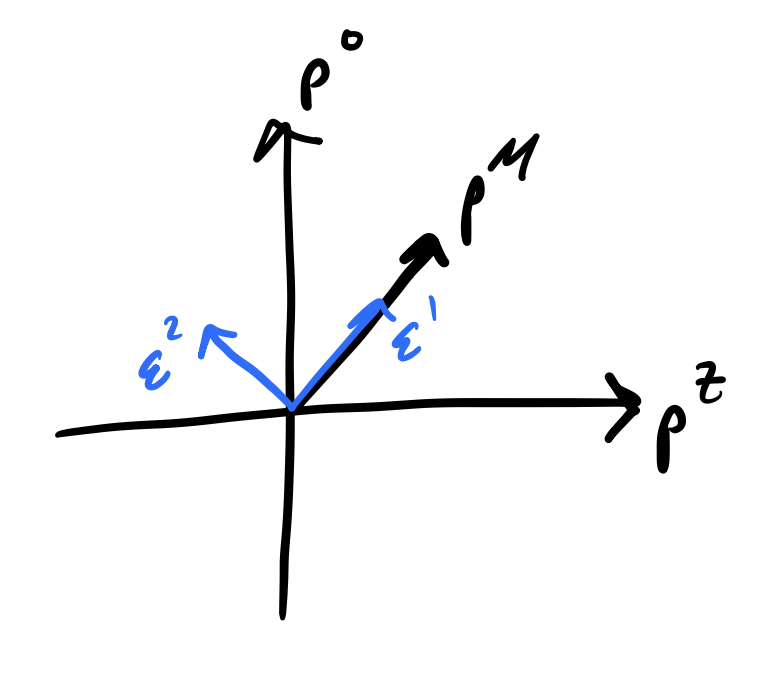
\includegraphics[scale=0.35]{Lectures/Images/lec12-unphysicalpolarizations.png}
\end{center}


So, the LSZ formula for $\gamma\gamma \to \gamma\gamma$ scattering is:
\begin{equation}
    \braket{f}{i} = i^4\int_{x_1x_2x_3x_4}e^{i(p_1x_2 + p_2x_2 - p_3x_3 - p_4x_4)}(\p_{x_1}^2\p_{x_2}^2\p_{x_3}^2\p_{x_4}^2)\e^{\mu_1}_{h_1}\e^{\mu_2}_{h_2}\e^{\mu_3}_{h_3}\e^{\mu_4}_{h_4}\avg{\mathcal{T}A_{\mu_1}(x_1)A_{\mu_2}(x_2)A_{\mu_3}(x_3)A_{\mu_4}(x_4)}
\end{equation}
Again this has a cleaner form when we Fourier transform:
\begin{equation}
    i\mathcal{M} = p_1^2p_2^2p_3^2p_4^2\e^{\mu_1}_{h_1}\e^{\mu_2}_{h_2}\e^{\mu_3}_{h_3}\e^{\mu_4}_{h_4}\avg{0}\mathcal{T}A_{\mu_1}(p_1)A_{\mu_2}(p_2)A_{\mu_3}(p_3)A_{\mu_4}(p_4)\ket{0}_c
\end{equation}
Much like in the scalar and fermion case, we have that the external legs are amputated.

\subsection{Do Photons Scatter?}
The simplest diagram that contributes to $\mathcal{M}$ looks like:

\begin{center}
    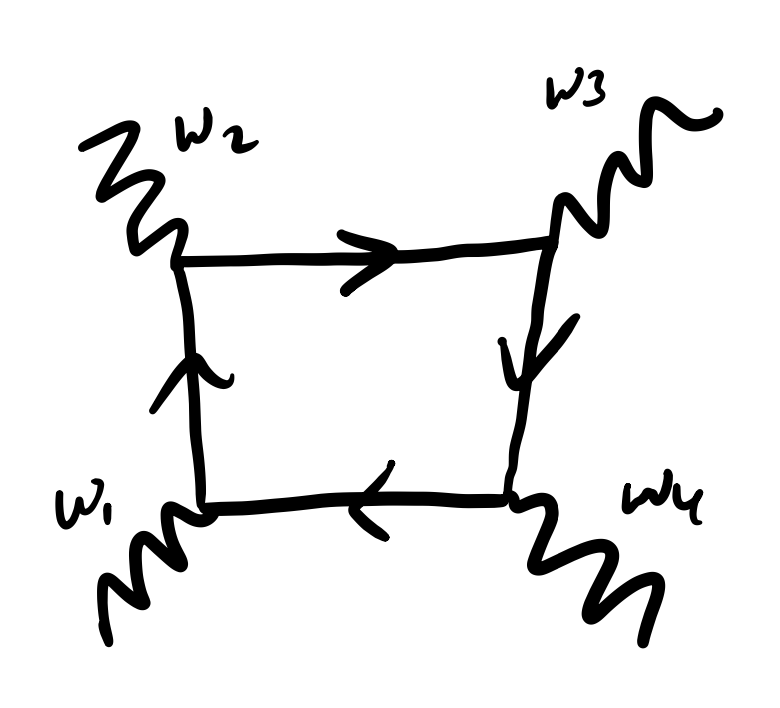
\includegraphics[scale=0.35]{Lectures/Images/lec12-photonscatterdiagram.png}
\end{center}


QED tells us that the superposition principle is incorrect; we have nonlinear effects that cause photons to scatter. But, this diagram is very small, so the superposition principle is approximately correct. Let's estimate how small this is. We have:
\begin{equation}
    \frac{m_ec^2}{\hbar} \sim 10^{21}\si{Hz}
\end{equation}
while visible light has:
\begin{equation}
    \omega \sim 10^{14}\si{Hz}
\end{equation}
the diagram goes as $\sim \frac{\omega^4}{m_e^4}\alpha^2 \sim 10^{-32}$.

In deriving the photon LSZ formula, we made a leap of faith, postulating the form of it assuming that there was a mass gap. But of course there is not. The approach we will take is to ignore it until we cannot ignore it - things will eventually go wrong. At tree level, scattering in QED looks fine. But once we start studying loops, things will not make sense. When we have loops, we have higher powers of the coupling, so we start including terms with more external photons, wherein we will have to return to this problem.